\ifdefined\included
\else
\documentclass[a4paper,11pt,twoside]{StyleThese}
\include{formatAndDefs}
\newcommand{\widthValue}{0.13\linewidth}
\sloppy
\begin{document}
\setcounter{chapter}{0} %% Num�ro du chapitre pr�c�dent ;)
\dominitoc
\dominilof
\faketableofcontents
\fakelistoffigures
\fi

\chapter{NMPC walking pattern generator}
\label{chap:nmpc}

\ifdefined\included
\else
\minitoc
\minilof
\fi

\cleardoublepage

%!TEX root = 16-ra-letter-NMPCWalkGen.tex

In the present chapter we present a real-time nonlinear model predictive control (NMPC) executable on the humanoid robot HRP-2.
This chapter has been developed in the frame of the collaborative project \koroibot\ and published in \cite{naveau:ral:2016}.
Following the idea of ``walking without thinking", we propose a walking pattern generator that takes into account simultaneously the position and orientation of the feet.
A requirement for an application in real-world scenarios is the avoidance of obstacles.
Therefore, an extension of the pattern generator that directly considers the avoidance of obstacles is derived.
The algorithm uses the whole-body dynamics to correct the center of mass trajectory of the underlying simplified model.
The pattern generator runs in real-time on the embedded hardware of the humanoid robot HRP-2 and experiments demonstrate the increase in performance with the correction.

In Sec.~\ref{Sec:nmpcmotivation} we present the motivation and the related works. Sec.~\ref{Sec:dynamic} is a reminder of the LIPM equation as well as the principles used in \cite{herdt:iros:2010}. Sec.~\ref{Sec:nmpc} depicts the formulation of the problem as a sequence of locally linearized quadratic problems and the real-time feasible solution by applying the idea of the so called "real-time" iteration.
A particular treatment of the dynamical filter is given in Sec.~\ref{Sec:dynamic_filter}.
Finally, our practical contribution, showing that the algorithm can be implemented in real-time on the humanoid robot HRP-2, is detailed in Sec.~\ref{sec:experiments_with_hrp2}.

\section{Introduction}

\subsection{Motivation}
\label{Sec:nmpcmotivation}

The recent DARPA robotics challenge have shown the need for humanoid robots with an increased level of functionality
enabled by proper control.
Such complex robots must provide a simple interface for humans and handle as much as possible the motion generation autonomously.
A general scheme is to use a motion planner to find an optimal path over a discrete set of foot-step transitions between two quasi-static poses \cite{Chestnutt:2010:MPHR,Hornung:ICHR:12}.
The foot-steps transition are given by a statistical exploration of a whole-body controller together with a walking pattern generator.
The planner then finds a feasible sequence of quasi-static poses and foot-step transitions which minimizes a cost function and avoids obstacles.
This solution is then improved online while ensuring feasibility, see for instance \cite{perrin:itro:12}.
In general it is not possible to realize real-time motion planning by directly using the controller itself because it is not possible to run more than one or two instances of the same controller before collision.
Therefore, when the planner fails it is necessary to solve a continuous local problem which will provide a feasible solution different from the precomputed one \cite{Chestnutt:2010:MPHR}.
The statistical exploration can be advantageously used to cast an optimization problem to find an initial guess \cite{Chestnutt:2010:MPHR}.
Recently, \emph{Deits} proposed to define the area of convergence for a local convex problem with linear constraints \cite{deits:ichr:14}
for a template model.
With template models the inertia related to the whole-body motion is ignored, regulated to zero or corrected.
In this chapter it is corrected by means of a dynamic filter. It is shown in the experimental section that it is drastically improving the 
performances over \cite{herdt:iros:2010} on the same robot.
The use of template model is a practical solution on platforms with limited computation capabilities.
%\todo{%
Even if advanced whole-body motion controllers are now closer to real-time feasibility, e.g. the one proposed by \emph{Todorov} which was recently applied to
HRP-2~\cite{Koenemann:iros:2015}, they still need powerful multi-core CPUs which limit their integration on humanoid robots due to heat and power consumption.
\begin{figure}[t]
  \centering
  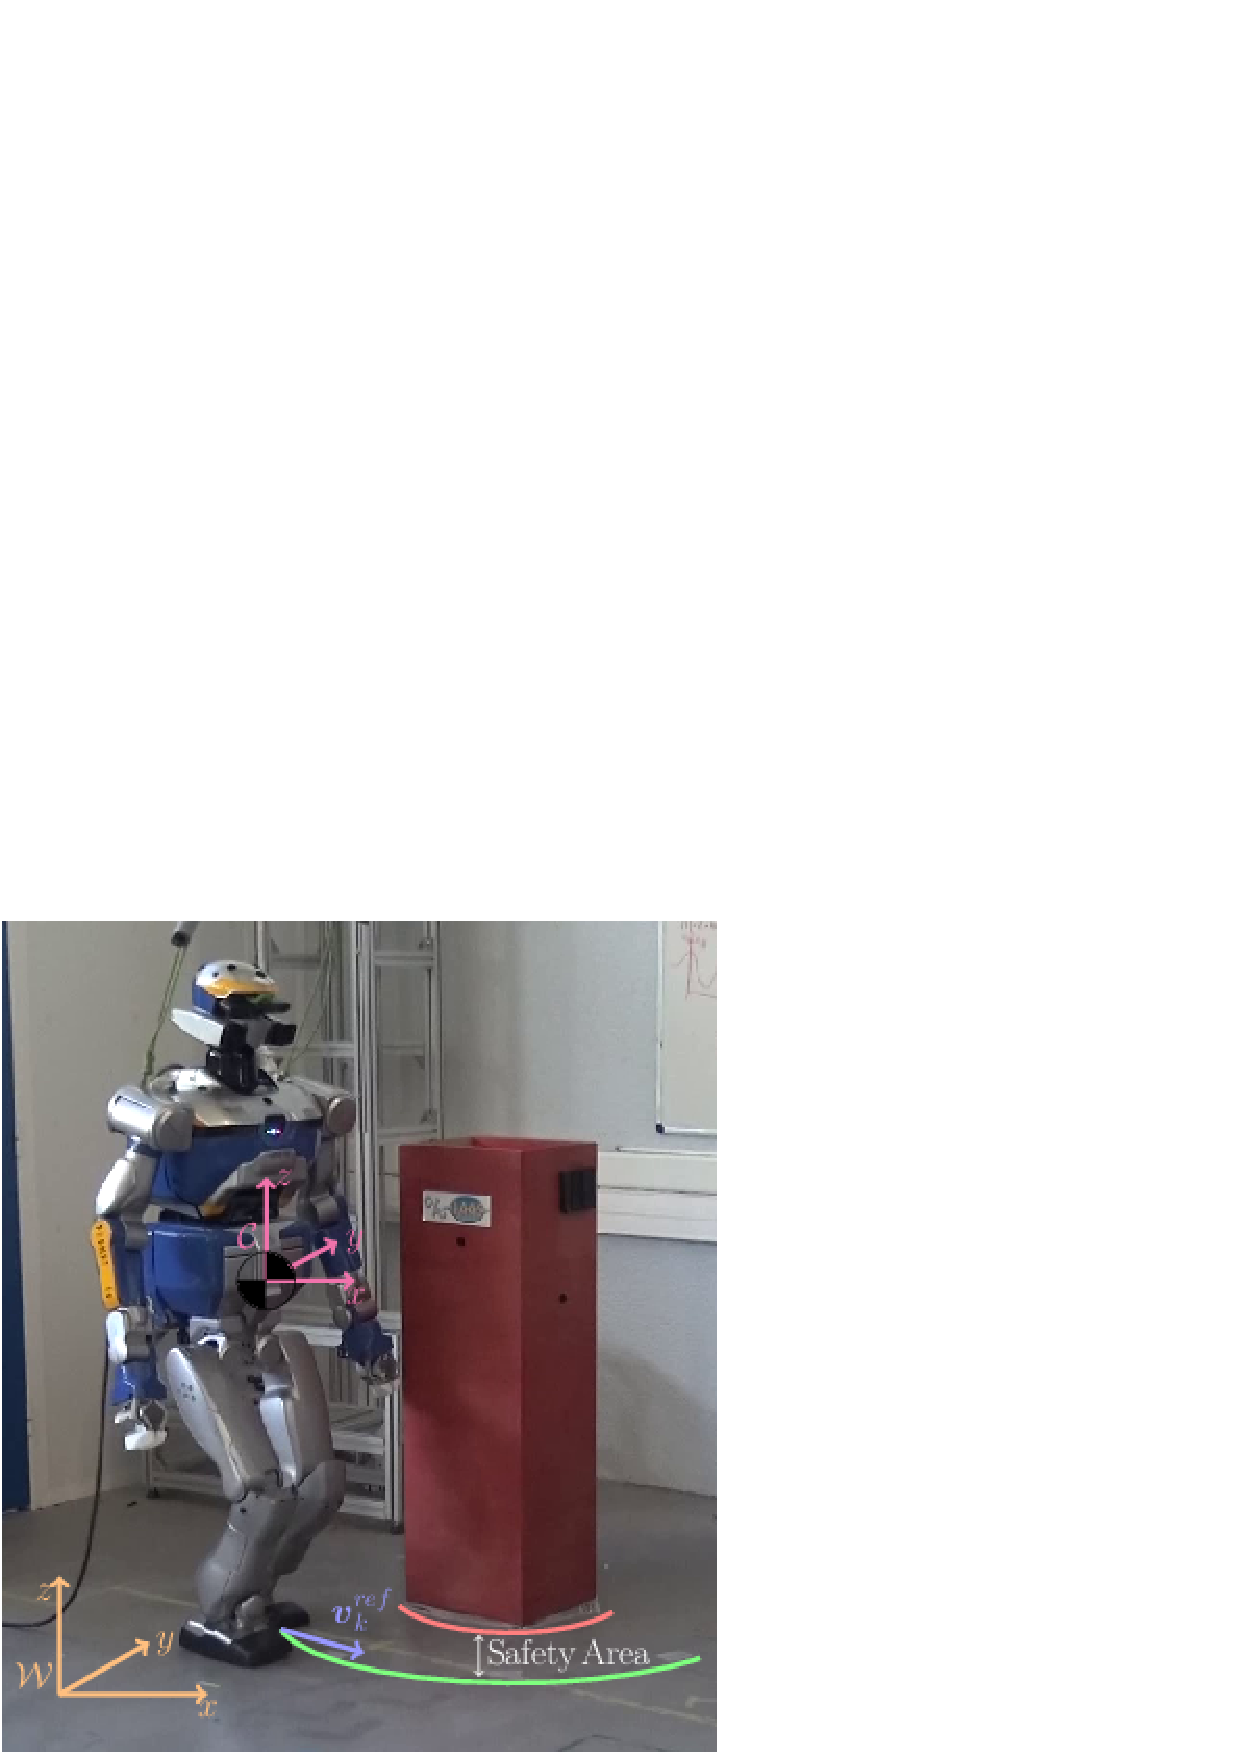
\includegraphics[width=0.4\linewidth, keepaspectratio]{synthesis.pdf}
  \caption[Problem setup]{HRP-2 avoiding reactively on an obstacle, even if the reference velocity $v^{ref}_k$ drives it into it. The upper body geometry is taken into account by setting a constraint (in green) such that the robot is sufficiently away from the obstacle (in red).}
  \label{fig:covernmpcwalkgen}
\end{figure}

Another improvement of this chapter over the method developed in \cite{herdt:iros:2010} is the nonlinear formulation which here allows to deal with obstacle.
More precisely \cite{herdt:iros:2010} integrates the information provided by statistical exploration of the controller feasibility 
between two foot-step transitions. It makes possible to correct foot-steps while having a guarantee over their feasibility.
%directly inside the walking pattern generator and is able to correct foot-steps. (MK: where is statistical exploration in the PG. Can you clarify? Is it a combination of planning and motion generation that you mean?)
%}
It is realized by reformulating the optimization problem to generate balanced Center-of-Pressure (CoP) and Center-of-Mass (CoM) trajectories where the free variables are the jerk of the CoM as well as foot-step positions and orientations.
The feasible foot-steps, i.e. free of self-collision and singularities, are specified through linear constraints.
This works well for level ground walking, unfortunately integrating obstacles with linear constraints implies a pre-processing of the environment or to use a different solver.

The present chapter shows that obstacles can be dealt with in real-time using a nonlinear scheme.
Although not demonstrated in this chapter, it can be coupled with a real-time planner.
The proposed method would provide a local feasible solution while the planner is looking for a global feasible solution \cite{perrin:itro:12}.
%For this reason, approaches with simple user input, e.g. the direction of walking and average velocity, have a high potential regarding real-world applications.
%This requires the robot to be able to find its foot steps and provide stability while walking autonomously.
%\todo{Furthermore, a highly capable controller lowers the burden of motion planners (MK: Do we use that?)}.

\subsection{Related work}
Previous works have proposed to apply Model Predictive Control (MPC) to humanoid robots walking by considering either the whole body or a template model.
When a model is available for a robot, MPC has several advantages.
It can be very fast when using analytical solutions \cite{Morisawa:ICRA:2007,Tedrake:ur:15,Faraji:ICRA:2014}.
However such formulation makes generally some specific assumptions to find the derivation.
This makes difficult the extension to other walking functionalities.
On the other hand 
MPC schemes formulated as an optimization problem  with a finer discretization grid can be more easily modified to include various walking modes 
inside a single formulation \cite{Sherikov:ichr:2014}.
In addition MPC as an optimization problem is becoming increasingly popular \cite{Feng:ichr:2013}, 
because for a given class of problems it allows using efficient off-the-shelf solvers.
Moreover several methods exist to increase the efficiency of solvers for NMPC problems.
For instance, it is possible to use warm-starts or use a sub-optimal solution while maintaining feasibility \cite{Boyd:CO:2004}.
The goal in humanoid robotics is to find a problem formulation which realizes all the needed functionalities and copes with the robot capabilities.
The locomotion problems described in \cite{mordatch:tog:12}, that include multi-contacts and consider the whole robot model over a time horizon, 
are not yet solvable in real-time and strongly depend on the models used to represent the physics.

Despite numerous efforts to address this large scale nonlinear problem with roughly ten thousand variables \cite{Koenemann:iros:2015,Dai:ICHR:2014}, no solution yet exists to generate physically consistent controls in real-time using humanoid robot embedded computers.
On the other hand template models projecting the overall robot dynamics to its CoM are used in research works \cite{Wensing:iros:2014,Orin:AURO:2012,Kajita:icra:2003,Englsberger:ichr:2015}, and already showing promising performance.
Motion generation with template models can sometimes be solved analytically, and in such cases provide fast solutions that are particularly well suited for platforms with limited computational power.
However, when increased CPU power is available, MPC-based solutions with the whole model are much more complete and reliable.
Furthermore, as they can be easily modified, they provide more adaptive functionalities.
In this chapter, with a bottom-up approach, we are trying to increase the functional level of a control architecture that already works on an existing humanoid robot, HRP-2 \cite{herdt:iros:2010}.
The point of this chapter is to present extensions of the linear MPC scheme presented in \cite{herdt:iros:2010}, that allows automatic foot placement in real-time.
For instance, the problem depicted in Fig.~\ref{fig:covernmpcwalkgen} shows the humanoid robot HRP-2 driven by a desired velocity provided by the user.
%\todo{%
The former scheme \cite{herdt:iros:2010} was specifically formulated as a cascade of two quadratic programs (QPs). Foot-step orientations are solution of the first problem, while the second solution of the second QP provides the CoM trajectory and foot-step positions. This separation is efficient because the constraints are linear.
%(say something about position and orientation?)}
If an obstacle has to be taken into account then the constraints have the shape depicted in Fig.~\ref{fig:algo_diff}, which is not convex anymore.
To maintain the convexity, the solution would be to pre-process the obstacle and the feasibility area of the foot-steps.
However a linearization of the obstacle boundary is equivalent to adding a linear constraint as depicted in Fig.~\ref{fig:algo_diff}.
The algorithm proposed in this chapter is doing a similar operation and therefore no pre-processing is necessary.
This is one of the major contribution of this chapter in comparison to \cite{herdt:iros:2010}.
The proposed nonlinear extension takes into account the exact expression of constraints such as, for instance, locally avoiding a convex obstacle.
Other formulations for walking motion generation have already been proposed.
\cite{deits:ichr:14} is using mixed-integer convex optimization for planning foot-steps with Atlas.
\cite{Ibanez:ark:14} is using mixed-integer convex optimization for MPC control and foot steps timing.
In this work we introduce three nonlinear inequalities to handle balance, foot step orientation and obstacle avoidance.
This new real time walking pattern generator has been successfully tested on the humanoid robot HRP-2 as depicted in Fig.~\ref{fig:covernmpcwalkgen}.
A key ingredient for achieving real-time performance was the following observation: \emph{one real-time iteration of the nonlinear scheme is enough to find a reasonable solution}.

\begin{figure}[ht]
    \centering
    %!TEX root = ../../14-icra-RealTimeNMPC.tex

\newcommand{\tetazero}{20.55}
\newcommand{\Fkxzero}{-20}
\newcommand{\Fkyzero}{20}

\newcommand{\tetaone}{-20}
\newcommand{\Fkxone}{5}
\newcommand{\Fkyone}{0}

\newcommand{\tetatwo}{20}
\newcommand{\Fkxtwo}{25}
\newcommand{\Fkytwo}{20}

%\includegraphics[width=15cm]{./figures/walking-without-thinking/ConvexHull}
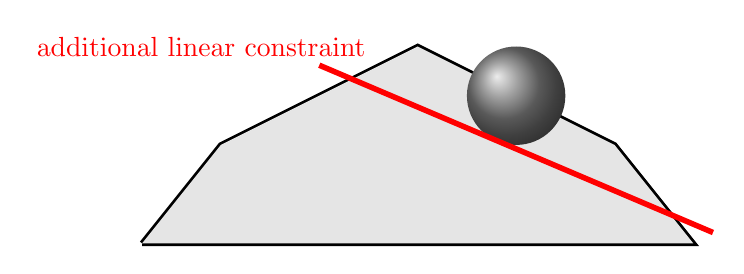
\begin{tikzpicture}[scale=0.125]
%\draw [dashed][->](-50,0) -- (50,0) node [below left, black]{$\overrightarrow{x}$}; %x-axis
%\draw [dashed][->](0,-50) -- (0,50) node [below left, black]{$\overrightarrow{y}$}; %y-axis
 %left support, right foot landing convexhull
\draw [line width=2pt](-28,20)--(-20,30)--(0,40)--(20,30)--(28,20)--(-28,20) node at (-10,30)[black]{} ;
\fill [color=gray!20,line width=2pt] (-28,20)--(-20,30)--(0,40)--(20,30)--(28,20)--(-28,20) ;
%pattern=north east lines
 %support foot
%\draw (-10,-5)--(10,-5)--(10,5)--(-10,5)--(-10,-5) node [below left, black]{Support Foot} ;

\shade[ball color=gray] (10,35) circle (5cm);

\draw [line width=2pt,red](-10,38.10)--(30,21.10) node at (-22,40)[red]{additional linear constraint} ;
\end{tikzpicture}

%
%\begin{tikzpicture}[x=0.7cm,y=0.7cm]
%\node (D) at (0,0) [coordinate] {} ;
%\node [below left] at (D) {D} ;
%\node (G) at (3,0) [coordinate] {} ;
%\node [below] at (G) {G} ;
%\node (C) at (5,0) [coordinate] {} ;
%\node [below right] at (C) {C} ;
%\node (F) at (5,3) [coordinate] {} ;
%\node [right] at (F) {F} ;
%\node (B) at (5,5) [coordinate] {} ;
%\node [above right] at (B) {B} ;
%\node (E) at (2,5) [coordinate] {} ;
%\node [above] at (E) {E} ;
%\node (A) at (0,5) [coordinate] {} ;
%\node [above left] at (A) {A} ;
%\node (H) at (0,2) [coordinate] {} ;
%\node [left] at (H) {H} ;
%\filldraw[color=lightgray] (D) -- (G) -- (H) ;
%\filldraw[color=lightgray] (G) -- (C) -- (F) ;
%\filldraw[color=lightgray] (F) -- (B) -- (E) ;
%\filldraw[color=lightgray] (E) -- (A) -- (H) ;
%\draw (D) -- node[below] {$b$} (G) -- node[below] {$a$} (C) ;
%\draw (C) -- node[right] {$b$} (F) -- node[right] {$a$} (B) ;
%\draw (B) -- node[above] {$b$} (E) -- node[above] {$a$} (A) ;
%\draw (A) -- node[left] {$b$} (H) -- node[left] {$a$} (D) ;
%\draw (G) -- (F) ;
%\draw (F) -- (E) ;
%\draw (E) -- (H) ;
%\draw (H) -- (G) ;
%\end{tikzpicture}
%
%
%
%
%\begin{tikzpicture}[x=0.7cm,y=0.7cm]
%\node (D) at (0,0) [coordinate] {} ;
%\node [below left] at (D) {D} ;
%\node (G) at (3,0) [coordinate] {} ;
%\node [below] at (G) {G} ;
%\node (C) at (5,0) [coordinate] {} ;
%\node [below right] at (C) {C} ;
%\node (F) at (5,3) [coordinate] {} ;
%\node [right] at (F) {F} ;
%\node (B) at (5,5) [coordinate] {} ;
%\node [above right] at (B) {B} ;
%\node (E) at (2,5) [coordinate] {} ;
%\node [above] at (E) {E} ;
%\node (A) at (0,5) [coordinate] {} ;
%\node [above left] at (A) {A} ;
%\node (H) at (0,2) [coordinate] {} ;
%\node [left] at (H) {H} ;
%
%\filldraw[color=lightgray,pattern=crosshatch] (G) -- (C) -- (F) ;
%\filldraw[color=lightgray,pattern=crosshatch] (F) -- (B) -- (E) ;
%\filldraw[color=lightgray,pattern=crosshatch] (E) -- (A) -- (H) ;
%\draw (D) -- node[below] {$b$} (G) -- node[below] {$a$} (C) ;
%\draw (C) -- node[right] {$b$} (F) -- node[right] {$a$} (B) ;
%\draw (B) -- node[above] {$b$} (E) -- node[above] {$a$} (A) ;
%\draw (A) -- node[left] {$b$} (H) -- node[left] {$a$} (D) ;
%\draw (G) -- (F) ;
%\draw (F) -- (E) ;
%\draw (E) -- (H) ;
%\draw (H) -- (G) ;
%\end{tikzpicture}

    \caption{Walkable zone distorted by a convex obstacle}
    \label{fig:algo_diff}
\end{figure}

\subsection{Contribution of the chapter}

%\textcolor{blue!70}{The contributions of this work are the following:
\begin{itemize}
\item It proposes a nonlinear reformulation of classical walking pattern generator able to find simultaneously foot-step positions and orientations.
\item It introduces nonlinear constraints able to cope with obstacles in the environment.
\item It shows experimentally that one iteration of the nonlinear iterative scheme provides a suboptimal but sufficient solution for practical cases.
\item Thanks to the use of a dynamical filter that corrects the CoM trajectory to compensate the limitation of the template model as in \cite{Nishiwaki:IJRR:09}
the whole body dynamics can be taken into account. This technical implementation has a strong impact on the robot performances.
\item The whole algorithm runs in real time on the embedded hardware of the human-size humanoid robot HRP-2.
\end{itemize}
To be completely fair we are not doing NMPC using sensor feedback on the walking pattern generator.
The feedback loop of the algorithm is done by the dynamic filter (see Fig.~\ref{fig:combined_feedback_scheme}).
In fact the sensor feedback is already done by the commercial stabilizer from Kawada Industry.
Additional ongoing work is done to close the loop but the stabilizer is a closed-source software.
Hence it is rather difficult to be exactly sure of its behavior.



% outline

%%\section{Linearization with two QPs}
%% \subsection{QP controller}
%%   \subsubsection{Orientation QP}
%%   \subsubsection{Position QP}
%% \subsection{The constraints}

%!TEX root = 16-ra-letter-NMPCWalkGen.tex
%\newcommand*\refeq[1]{#1}
%\newcommand*\rfrac[2]{{}^{#1}\!/_{#2}}

\section{Derivation of the dynamics}
\label{Sec:dynamic}

In this work the well known Linear Inverted Pendulum Model (LIPM) from \cite{Kajita:icra:2003} is used as the template model of the robot's dynamics 
and the following assumptions are made:
1) the angular momentum produced by the rotations of all the robot parts is supposed to be zero,
2) the robot CoM evolves on a horizontal plane,
3) the normals of the contact forces have to be collinear.
As a consequence, each quantity can be expressed as a function of three degrees of freedom (DoFs), which are the projection of the robot CoM $(x,y)$-position on the ground plane and its free-flyer orientation $\theta$ around the vertical axis $z$.
The reader is kindly referred to \cite{herdt:iros:2010} for a detailed description of the several terms omitted for a sake of clarity in the following section.

\subsection{Discretization of CoM dynamics}
\label{SubSec:comDiscr}

In order to obtain a smooth trajectory, one controls the robot CoM through its jerk $\dddot{c}^{\nu}$ on a preview horizon, where $c$ denotes the position of the CoM in the world frame and $\nu \in \{ x, y \}$
%\footnote{In this algorithm the CoM height is constant, i.e. ${c}^{z}\equiv const.$}
is used to simplify the notation.
This is done by applying a constant sampling period $T$ and by assuming a piecewise constant jerk on each interval, i.e. $\dddot{c}_{k}^{\nu}(t) \equiv constant$, $t \in \left[k T, (k+1) T \right]$, $k\in\{0, 1, ..., N\}$, where $N$ is the length of the preview horizon.

The following time-stepping scheme maps the current state of the frame $c_k^{\nu}$ to the future states by
\begin{equation}
  \label{eq:com_der}
  \hat{c}_{k+j}^{\nu} = A^j \, \hat{c}_{k}^{\nu} \;+\; \sum_{i=0}^{j-1}{A^{i}\,B\,
  \dddot{c}^{\nu}_{k+i}}
  \,\,\, , \,\,\, j \in [0,N] ,
\end{equation}
\vspace*{-0.24cm}
\begin{equation}%\scriptstyle
\label{eq:time_scheme}
    \hat{c}_{k}^{\nu} =
    \begin{bmatrix}
        c_{k}^\nu \\
        \dot c_{k}^\nu\\
        \ddot c_{k}^\nu
    \end{bmatrix},\
    A =
    \begin{bmatrix}
        1 & T & \rfrac{T^2}{2} \\
        0 & 1 & T \\
        0 & 0 & 1
    \end{bmatrix},\
    B =
    \begin{bmatrix}
        \rfrac{T^3}{6} \\
        \rfrac{T^2}{2} \\
        T
    \end{bmatrix}.
\end{equation}
To express the CoM over the preview horizon the vector $C_{k+1}^\nu$ of size $\mathcal{R}^N$ and its derivatives are defined as
\begin{align}
  &C_{k+1}^\nu =
  \begin{bmatrix}
    c_{k+1}^\nu &
    \hdots &
    c_{k+N}^\nu \notag
  \end{bmatrix}^T
  ,
\;%\\
  &\dot{C}_{k+1}^\nu =
  \begin{bmatrix}
    \dot{c}_{k+1}^\nu &
    \hdots &
    \dot{c}_{k+N}^\nu \notag
  \end{bmatrix}^T
  ,
\\
  &\ddot{C}_{k+1}^\nu =
  \begin{bmatrix}
    \ddot{c}_{k+1}^\nu &
    \hdots &
    \ddot{c}_{k+N}^\nu \notag
  \end{bmatrix}^T
  ,
\;%\\
 &\dddot{C}_{k+1}^\nu =
  \begin{bmatrix}
    \dddot{c}_{k+1}^\nu &
    \hdots &
    \dddot{c}_{k+N}^\nu \notag
  \end{bmatrix}^T
  .
\end{align}
Using eq.~(\ref{eq:com_der}), the above vectors can be expressed as a function of the initial state $\hat{c}_k^\nu$ and the CoM jerk
$
\dddot{C}_{k+1}^\nu
%=
  % \begin{bmatrix}
  %   \dddot{c}_{k+1}^\nu &
  %   \hdots &
  %   \dddot{c}_{k+N}^\nu \notag
  % \end{bmatrix}^T
$.
The latter belongs to the free-variable vector of the optimization problem described in section~\ref{Sec:nmpc}.

\subsection{Linear inverted pendulum dynamics}
\label{SubSec:LIPM}

In this chapter the balance criteria used is the one that have the center of pressure (CoP) in the convex hull of the robot's support polygon, which is defined by the contacts with the ground
\cite{Kajita:icra:2003} (see Sec.~\ref{SubSec:constraints}).
Hence, the CoP has to be expressed in terms of the system's free variables, i.e. the CoM jerk.
Using the assumptions made in the introduction of Sec.~\ref{Sec:dynamic}, the robot CoP can be expressed as a linear function of the CoM, i.e.
\begin{equation*}
    z_{k+n}^{\nu} =
    \begin{bmatrix}
        1 & 0 & -\rfrac{h}{g}
    \end{bmatrix} \hat{c}_{k+n}^\nu
    \, , \,\,\, \nu \in \left\{ x,y \right\}
    , n \in [0,N-1]
    ,
\end{equation*}
with $h=c^z-z^z$ being the height of the CoM with respect to the ground and $g$ the norm of the gravity vector.
Using eq.~\eqref{eq:com_der}, a recursive expression for the future evolution of the CoP for a fixed horizon of $N$ sampling steps  is given by
\begin{equation}
    \label{eq:zmp_horizon}
   	z_{k+n}^{\nu} =
   	\begin{bmatrix}
        1 & 0 & -\rfrac{h}{g}
    \end{bmatrix} \left[ A^n \, \hat{c}_{k}^{\nu} \;+\; \sum_{i=0}^{n-1}{A^{i}\,B\,
  \dddot{c}^{\nu}_{k+i}} \right]
  .
\end{equation}
As in Sec.~\ref{SubSec:comDiscr}, the vector
$	Z_{k+1}^\nu =
    \begin{bmatrix}
        z_{k+1}^\nu &
        \hdots &
        z_{k+n}^\nu \notag
  \end{bmatrix}^T$~,
of size $\mathcal{R}^N$, is used to describe the CoP on the preview horizon.
This vector can then be expressed in terms of $\hat{c}_k^\nu$
and $\dddot{C}_{k+1}^\nu$.

\subsection{Automatic foot step placement}
\label{SubSec:automaticFootPlacement}

The adaptive placement of the feet, with the aim to ensure balance of the robot even under external perturbations, is a key-feature of the algorithm.
To this end, consider a frame $\mathcal F$ attached to the support foot, with its current position and orientation on the ground given by $f_k^\eta$, with $\eta \in \{x,y,\theta\}$.
The future steps, also free variable of the optimization problem, are denoted by
\begin{align}
&F_{k+1}^\eta =
    \begin{bmatrix}
        f^\eta_{k+1} &
        f^\eta_{k+2} &
        \hdots &
        f^\eta_{k+N}         	
    \end{bmatrix}^T
    \notag \\
    	\label{eq:Fkp1}
&F_{k+1}^\eta = v_{k+1} f_{k}^{\eta} + V_{k+1} \tilde{F}_{k+1}^{\eta}
\end{align}
with $F_{k+1}^\eta$ of size $\mathcal{R}^N$ representing the foot support position at each time step and $\tilde{F}_{k+1}^\eta$ of size $\mathcal{R}^{nf}$ the actual free variables of the problem.
The vector $v_{k+1} \in \R^N$ and matrix $V_{k+1} \in \R^{N\times nf}$ indicate which step falls in which sampling interval (see \cite{herdt:iros:2010} for more details).
Sampling times correspond to rows, steps to columns, and $nf$ is the maximum number of double support phases in the preview.

In theory, the usage of a single point mass as model prevents the definition of an orientation.
In \cite{herdt:iros:2010} a frame attached to the center mass is defined and the orientation of this frame and the feet directions are optimized.
In this work only the foot step orientations are optimized, and the orientation of the robot free-flyer is computed from this solution.
Let $\text{ff}^{\theta}(t)$, $f^{\theta,L}(t)$ and $f^{\theta,R}(t)$ be respectively the orientation of the free-flyer, the left foot and the right foot at any time $t$.
Hence $\text{ff}^{\theta}(t)$ is by convention :
\begin{align*}
\begin{bmatrix}
	\text{ff}^{\theta}(t) \\
	\dot{\text{ff}}^{\theta}(t) \\
	\ddot{\text{ff}}^{\theta}(t)
\end{bmatrix}
=
\begin{bmatrix}
	\frac{1}{2}(f^{\theta,L}(t)        + f^{\theta,R}(t)) \\
	\frac{1}{2}(\dot{f}^{\theta,L}(t)  + \dot{f}^{\theta,R}(t)) \\
	\frac{1}{2}(\ddot{f}^{\theta,L}(t) + \ddot{f}^{\theta,R}(t))
\end{bmatrix}
.
\end{align*}

%%%%%%%%%%%%%%%%%%%%%%%%%%%%%%%%%%%%%%%%%%%%%%%%%%%%%%%%%%%%%%%%%%%%%%%%%%%%%%%%%%%%%%%%%%%%%%%%%%%%%%%%%%%%%%%%%%%%%%%%%%%%%%%%%%%%%%%%%%%%%%%%%%%%%%%%%%%%%%%%%%%%%%%%%%%%%%%%%%%%%%%%%%%%%%

\section{Nonlinear Model Predictive Control}
\label{Sec:nmpc}

Solving the orientation problem separately from the position problem is a workaround to linearize the CoP (eq.~\eqref{eq:zmpCanonicConstraint}) and foot position (eq.~\eqref{eq:footCanonicConstraint}) constraints derived below.
However, computing separately the orientation and then injecting the solution into the position QP amounts to solve a different problem than the nonlinear combination of both.
In the following the nonlinear problem will be derived and analyzed, and an appropriate approach allowing the real-time execution of the algorithm on the robot will be proposed.

\subsection{The controller}
\label{SubSec:controller}

\begin{figure}[h]
    \centering
    %!TEX root = ../../14-icra-RealTimeNMPC.tex

\tikzstyle{block} = [draw, fill=blue!20, rectangle,
    minimum height=2em, minimum width=5em, align=center]
\tikzstyle{sum} = [draw, fill=blue!20, circle, node distance=1cm]
\tikzstyle{input} = [coordinate]
\tikzstyle{output} = [coordinate]
\tikzstyle{pinstyle} = [pin edge={to-,thin,black}]

% The block diagram code is probably more verbose than necessary
\begin{tikzpicture}[auto, node distance=2cm,>=latex]
    % We start by placing the blocks
    \node [input]  at (-1.5, 0.0) (input)  {};
    \node [input]  at (-0.5, -1.0) (feedback)  {};
    \node []    at ( 0.0, 0.0) (sumin)  {};
    \node [output]    at ( 14, 0.0) (sumout) {};

    \node [block] at (0.8,0) (wpg) {
        Walking\\
        Pattern\\
        Generator
    };
    \node [block] at (3.8,0) (dyn) {
        Dynamic\\
        Filter
    };
    \node [block] at (7.0,0) (sot) {
        Generalized\\
        Inverse\\
        Kinematics
    };
    \node [block] at (10.5, 0) (system) {
    		Robot Hardware\\
    		{\small Simulation/Robot}
    	};

    % PATHS
    	% Forward chaine
    \draw [draw,->] (input) -- node {\small ${Vel}^{\,ref}$} (wpg);
    \draw [draw,->] (wpg) -- node [text width=0.7cm]{\small $c^{ref}$ $f^{ref}$} (dyn);
    \draw [draw,->] (dyn.east) -- node [text width=0.7cm]{\small $\tilde{c}^{\,ref}$ $f^{ref}$} (sot);
    \draw [draw,->] (sot) -- node [text width=0.7cm]{\small $q^{ref}$ $\dot q^{ref}$} (system);
    %\draw [->] (system) -- node {} (sumout);

    % Feedback chaine
    \draw [- ] ($(dyn.east) + (0.35,0.0)$)  |- node {} (feedback);
    \draw [->] (feedback) |- node {} ([yshift=-0.2cm]wpg);

%    \draw [->] (dyn) -| node[above right] {\small $\hat{c}^{\,x,y,\theta}$, $\hat{f}^{\,\,x,y,\theta}$} (wpg);
\end{tikzpicture}


% The block diagram code is probably more verbose than necessary
%\begin{tikzpicture}[auto, node distance=2cm,>=latex']
%    % We start by placing the blocks
%    \node [input]  at (-0.5, 0.0) (input)  {};
%    \node [sum]    at ( 0.5, 0.0) (sumin)  {};
%    \node [sum]    at ( 6.5, 0.0) (sumout) {};
%    \node [output] at ( 7.5, 0.0) (output) {};
%
%    % QP Controller Blocks
%    \node [block] at (2.0,0) (oriqp) {
%        QP Controller\\
%        \small{Orientation}
%    };
%    \node [block] at (5.0,0) (posqp) {
%        QP Controller\\
%        \small{Position}
%    };
%    \node [block] at (5.0, -2.0) (dynamics) {Dynamics};
%    \node [block] at (2.0, -2.0) (system)   {System};
%
%    % PATHS
%    \draw [draw,->] (input) -- node {$
%        \dot C_{k+1}^{ref}
%    $} (sumin);
%    \draw [->] (oriqp) -- node {$U_k$} (posqp);
%    \draw [->] (posqp) -- node {$U_k$} (sumout);
%    \draw [->] (dynamics) --  (system);
%
%    \draw [->] (sumout) -- node {$ $} (output);
%    \draw [->] (sumin) -- node {} (oriqp);
%    \draw [->] (sumout) |- node[near start] {$y$}   (dynamics);
%    \draw [->] (system) -| node[near end]   {$val$} (sumin);
%\end{tikzpicture}

    \caption[Control scheme]{The control scheme: ${Vel}^{\,ref}$ is the input velocity.
     $c^{ref}$ and $f^{ref}$ are respectively the CoM and the feet 3D trajectories
     $\tilde{c}^{\,ref}$ is the CoM trajectory filtered.
     $q^{ref}$, $\dot q^{ref}$ denote respectively the generalized coordinate vector and its derivation.
     }
    \label{fig:combined_feedback_scheme}
\end{figure}

A scheme of the controller is shown in Fig.~\ref{fig:combined_feedback_scheme}.
This open-loop controller is used for tracking respectively a referenced linear and angular velocity.
In the first step, the walking pattern generator (WPG) computes the foot steps and CoM jerk from the given velocity
$ {Vel}^{\,ref}_{k+1} =$~$
\begin{bmatrix}
{Vel}_{k+1}^{x,ref} & {Vel}_{k+1}^{y,ref} & {Vel}_{k+1}^{\theta,ref}
\end{bmatrix} $.
Then it uses an Euler integration scheme to compute the CoM trajectory from its jerk and polynomials of fifth order to retrieve 3D trajectories for the feet from the foot step planning.
The CoM computed by the WPG is then filtered (see Sec.~\ref{Sec:dynamic_filter}) and sent altogether with the feet trajectory to a generalized inverse kinematics algorithm.
The output is a whole-body walking trajectory that can be applied directly on the robot.
The WPG is then reinitialized with the current reference velocity input and with the corrected initial states of the dynamic filter.

\subsection{The cost function}
\label{SubSec:costFunction}

The cost function used in the NMPC is given by
\begin{equation}
    \min_{U_{k}} \frac{\alpha}{2} J_1(U_k)
               + \frac{\alpha}{2} J_2(U_k)
               + \frac{\beta}{2}  J_3(U_k)
               + \frac{\gamma}{2} J_4(U_k)
\end{equation}
%\todo{Why do $J_1$ and $J_2$ use the same weight?}
%Simultaneously both the orientation and position of the foot steps need to be optimized.
with $\alpha$, $\beta$ and $\gamma$ being the weights of the cost function and $U_k$ the free variables of the problem defined as
\begingroup\makeatletter\def\f@size{9}\check@mathfonts
\def\maketag@@@#1{\hbox{\m@th\large\normalfont#1}}%
\begin{align}
  U_k^{x,y} =
  \begin{bmatrix}
    \dddot C_{k}^x &
    \tilde{F}_k^x  &
    \dddot C_{k}^y &
    \tilde{F}_k^y
  \end{bmatrix}^T
, \;\;\;\;
  U_k^{\theta} \,= \tilde{F}_k^{\theta}
, \;\;\;\;
  U_k =
  \begin{bmatrix}
    U_k^{x,y} &
    U_k^{\theta}
  \end{bmatrix}^T
  \label{eq:Uk}
  .
\end{align}
\endgroup
$J_1(U_k)$ is the cost function related to the linear velocity tracking
\begin{equation}
  J_1(U_k) = \lVert \dot C_{k+1}^{x} - {Vel}_{k+1}^{x,ref} \rVert^2_2
  +  \lVert \dot C_{k+1}^{y} - {Vel}_{k+1}^{y,ref} \rVert^2_2 \nonumber
  .
\end{equation}
$J_2(U_k)$ is the cost function related to the angular velocity tracking
\begin{equation}
  J_2(U_k) = \lVert F_{k+1}^\theta - \int {Vel}_{k+1}^{\theta,ref} dt \; \rVert_2^2 \nonumber
  .
\end{equation}
Experiments have shown that a different weight between linear and angular velocities was not necessary at this stage.
$J_3(U_k)$ is the cost function minimizing the distance between the CoP and the projection of the ankle on the sole
\begin{equation}
  J_3(U_k) = \lVert F_{k+1}^{x} - CoP_{k+1}^{x} \rVert^2_2 +
             \lVert F_{k+1}^{y} - CoP_{k+1}^{y} \rVert^2_2 
             .
\label{eq:cost_function_dist_to_copref}
\end{equation}
$J_4(U_k)$ is the cost function minimizing the norm of the control
\begin{equation}
  J_4(U_k) = \lVert \dddot C_{k+1}^{x} \rVert^2_2
           + \lVert \dddot C_{k+1}^{y} \rVert^2_2
    \nonumber
    % \label{eq:costFunction}
    .
\end{equation}
The above minimization function can then be express in a canonical form
\begin{align}
  &\min_{U_k} \quad \frac{1}{2} \;\; U_{k}\,^T \;Q_k \;U_{k} \;\;+\;\; p_k\,^T \;U_{k} \;,\\
\text{with } Q_k &=
\begin{bmatrix}
Q^{x,y}_k & 0  \\
 0        & Q_k^{\theta}
\end{bmatrix}, \;\;\;
p_k =
\begin{bmatrix}
p_k^{x,y} \\
p_k^{\theta}
\end{bmatrix}, \;\;\;
Q_k^{\theta} = \alpha \;\mathbb{I}_{nf}, \notag\\
p_k^{\theta} &= \alpha \left(
    \begin{bmatrix}
    1&\hdots&nf
    \end{bmatrix} \;
    T_{step} \; {Vel}_{k+1}^{\theta,ref} +
    \begin{bmatrix}
    1\\\vdots\\1
    \end{bmatrix}f_{k}^\theta \right)
    .\notag
\end{align}
The reader is kindly referred to \cite{herdt:iros:2010} for the defintion of $Q^{x,y}$ and $p^{x,y}$.
The matrix $Q_k^{\theta}$ and $p_k^{\theta}$ are derived because we use a slightly different method than \cite{herdt:iros:2010} to deal with the orientation.

\subsection{The constraints}
\label{SubSec:constraints}
First of all the balance of the robot has to be ensured, then the feasibility of the foot step needs to be verified.
Finally, the nonlinear constraint which implements the obstacle avoidance is described. It is one of the contribution introduced by this chapter.
The following exposition is based on \cite{herdt:iros:2010}.

\subsubsection{Balance constraint}
\label{seq:Constraints}

\begin{figure}[ht]
    \centering
    \scalebox{.8}{%!TEX root = ../../14-icra-RealTimeNMPC.tex

\newcommand{\tetazero}{20.55}
\newcommand{\Fkxzero}{-20}
\newcommand{\Fkyzero}{20}

\newcommand{\tetaone}{-20}
\newcommand{\Fkxone}{5}
\newcommand{\Fkyone}{0}

\newcommand{\tetatwo}{20}
\newcommand{\Fkxtwo}{25}
\newcommand{\Fkytwo}{20}

%\includegraphics[width=15cm]{./figures/walking-without-thinking/ConvexHull}
\begin{tikzpicture}[scale=0.050, node distance=2cm,>=latex]
\draw [->](-50,0) -- (60,0) node [below left, black]{$\overrightarrow{x}$}; %x-axis
\draw [->](0,-30) -- (0,40) node [below left, black]{$\overrightarrow{y}$}; %y-axis
 %support foot
\draw (-40,-20)--(40,-20)--(40,20)--(-40,20)--(-40,-20);

\draw [thick][dashed][->](0,0) -- (40,20) node [right, black]{${\bf p}_1$}; %y-axis
\draw [thick][dashed][->](0,0) -- (-40,20) node [left, black]{${\bf p}_2$}; %y-axis
\draw [thick][dashed][->](0,0) -- (-40,-20) node [left, black]{${\bf p}_3$}; %y-axis
\draw [thick][dashed][->](0,0) -- (40,-20) node [right, black]{${\bf p}_4$}; %y-axis

% rotated support foot
\draw [dotted][cm={cos(\tetazero) ,sin(\tetazero) ,-sin(\tetazero) ,cos(\tetazero) ,(0.0 cm,0.0 cm)}]
(-40,-20)--(40,-20)--(40,20)--(-40,20)--(-40,-20) ;
% rotated axis
\draw [dotted][-][cm={cos(\tetazero) ,sin(\tetazero) ,-sin(\tetazero) ,cos(\tetazero) ,(0.0 cm,0.0 cm)}]
(0,0) -- (40,0) node [below left, black]{};
% angle
\draw (0,0) -- (28.090986571,10.432619456) arc (\tetazero:0:30) -- (0.0,0.0) node at (32,6) {$\theta$} ;

\end{tikzpicture}
}
    \caption[Balance constraint]{Shape of the foot with the position vector $ {p}^z_{i} $ describing the support polygon and $ \theta $ representing its orientation.
    The $4\times2$ matrix $A_{cop}$ and the $4\times1$ vector $B_{cop}$ are the linear algebra representation of the edges.}
	\label{fig:foot}
\end{figure}

The CoP has to remain inside the support polygon \cite{Wieber:IWFFFR:2002}.
This polygon is depicted in Fig.~\ref{fig:foot}.
The set of linear inequalities representing the convex polygon is denoted as $A_{cop}$ and $B_{cop}$.
Only one foot is modeled as a support polygon for two reasons:
1) HRP-2 feet are symmetrical, 2) the sampling period of the problem is designed in a way that no iteration of the optimization problem falls into a double support phase.
The CoP at instant $k$, \mbox{($z_k = [z_k^x \;\; z_k^y]^T$)}, see Sec.~\ref{SubSec:LIPM}) lies inside the support polygon if and only if
\begin{align}
  A_{cop} R(f_k^\theta) \left( {z}_k - f_k
  \right) \leq B_{cop} \\
  \left[A_{cop,k}^{x,\theta} \;\;\;\;  A_{cop,k}^{y,\theta} \right] \left( {z}_k - f_k
  \right) \leq B_{cop} \\
  R(f_k^{\theta} ) =
  \begin{bmatrix}
  \cos(f_k^\theta) & \sin(f_k^\theta)\\
  -\sin(f_k^\theta) & \cos(f_k^\theta)
  \end{bmatrix}
  ,
\end{align}
where $f_k = [f_k^x \;\; f_k^y]^T$, $A_{cop,k}^{x,\theta}$ is the left column of $A_{cop} R(f_k^\theta)$ and $A_{cop,k}^{y,\theta}$ is the right one.
Using eq.~\eqref{eq:Fkp1} the constraint for each time step of the preview horizon is defined by
\begin{equation}
\label{eq:cop_constraint_extended}
D_{k+1}(U_k^\theta)
\begin{bmatrix}
Z_{k+1}^x - v_{k+1} f_{k}^x - V_{k+1} \tilde{F}_{k+1}^x \\
Z_{k+1}^y - v_{k+1} f_{k}^y - V_{k+1} \tilde{F}_{k+1}^y
\end{bmatrix} \leq
b_{cop}\,_{k+1}
\end{equation}
With $b_{cop}\,_{k+1} = [B_{cop} \hdots B_{cop}]^T$ and $D_{k+1}(U_k^\theta) = $
\begin{equation*}
\begin{bmatrix}
A_{cop,k+1}^{x,\theta} & & 0 & A_{cop,k+1}^{y,\theta} & & 0 \\
 & \ddots & & & \ddots \\
0 & & A_{cop,k+N}^{x,\theta} & 0 & & A_{cop,k+N}^{y,\theta} \\
\end{bmatrix}
.
\end{equation*}
From eq.~(\ref{eq:cop_constraint_extended}), the canonical form of the constraint is
\begin{equation}
A_{cop,k}(U_k^\theta) \; U^{x,y}_{k} \;\leq\; \overline{U_{cop,k}}
,
\label{eq:zmpCanonicConstraint}
\end{equation}
where $A_{cop,k}(U_k^\theta)$ is a matrix depending on $ U_k^\theta $ which makes this constraint nonlinear.
And $\overline{U_{cop,k}}$ is the upper bound vector. %symbolized with the over line.
The last steps of the derivation are detailed in \cite{herdt:iros:2010}.

\begin{figure}[ht]
    \centering
    %!TEX root = ../../14-icra-RealTimeNMPC.tex

\newcommand{\tetazero}{20.55}
\newcommand{\Fkxzero}{-20}
\newcommand{\Fkyzero}{20}

\newcommand{\tetaone}{-20}
\newcommand{\Fkxone}{5}
\newcommand{\Fkyone}{0}

\newcommand{\tetatwo}{20}
\newcommand{\Fkxtwo}{25}
\newcommand{\Fkytwo}{20}

%\includegraphics[width=15cm]{./figures/walking-without-thinking/ConvexHull}
\begin{tikzpicture}[scale=0.075]
\draw [dashed][->](-50,0) -- (50,0) node [below left, black]{$\overrightarrow{x}$}; %x-axis
\draw [dashed][->](0,-41) -- (0,50) node [below left, black]{$\overrightarrow{y}$}; %y-axis
 %right support, left foot landing convexhull
\draw (-28,-20)--(-20,-30)--(0,-40)--(20,-30)--(28,-20)--(-28,-20) node [below left, black]{$A_r$,$B_r$} ;
 %left support, right foot landing convexhull
\draw (-28,20)--(-20,30)--(0,40)--(20,30)--(28,20)--(-28,20) node at (-10,30)[black]{$A_l$,$B_l$} ;
 %support foot
\draw (-10,-5)--(10,-5)--(10,5)--(-10,5)--(-10,-5) node [below left, black]{Support Foot} ;

% rotated support foot
\draw [dotted][cm={cos(\tetazero) ,sin(\tetazero) ,-sin(\tetazero) ,cos(\tetazero) ,(0.0 cm,0.0 cm)}]
(-10,-5)--(10,-5)--(10,5)--(-10,5)--(-10,-5) ;
% rotated axis
\draw [dotted][-][cm={cos(\tetazero) ,sin(\tetazero) ,-sin(\tetazero) ,cos(\tetazero) ,(0.0 cm,0.0 cm)}]
(0,0) -- (30,0) node [below left, black]{};
% angle
\draw (0,0) -- (18.727324381,7.02049297) arc (\tetazero:0:20) -- (0.0,0.0) node at (21,5) {$\theta$} ;
% rotated left support, right foot landing convexhull
\draw [dotted][-][cm={cos(\tetazero) ,sin(\tetazero) ,-sin(\tetazero) ,cos(\tetazero) ,(0.0 cm,0.0 cm)}]
(-28,20)--(-20,30)--(0,40)--(20,30)--(28,20)--(-28,20) ;
% rotated right support, left foot landing convexhull
\draw [dotted][-][cm={cos(\tetazero) ,sin(\tetazero) ,-sin(\tetazero) ,cos(\tetazero) ,(0.0 cm,0.0 cm)}]
(-28,-20)--(-20,-30)--(0,-40)--(20,-30)--(28,-20)--(-28,-20);

\draw [thick][dashed][->](0,0) -- (-28,20) node [black] at (-33.0,20.0){${p}_1^l$}; %y-axis
\draw [thick][dashed][->](0,0) -- (-20,30) node [black] at (-25.0,32.0){${p}_2^l$}; %y-axis
\draw [thick][dashed][->](0,0) -- (0.0,40) node [black] at (5.0,42.0){${p}_3^l$}; %y-axis
\draw [thick][dashed][->](0,0) -- (20,30) node [right, black]{${p}_4^l$}; %y-axis
\draw [thick][dashed][->](0,0) -- (28,20) node [right, black]{${p}_5^l$}; %y-axis

\end{tikzpicture}

    \caption[Foot position constraint]{Shape of the selected convex polygon boundary of the foot placement. The $5\times2$ matrix $A_\textup{r,l}$ and the $5\times1$ vector $B_\textup{r,l}$, define the convex hull as a set of linear inequalities.}
	\label{fig:convexHull}
\end{figure}

\subsubsection{Foot step feasibility constraint}
\label{Sec:constraintOnFootPlacement}

This constraint uses the same convex hull as in \cite{herdt:iros:2010} to ensure the feasibility of the steps \cite{perrin2010approximation}.
For HRP-2 this convex hull is shown in Fig.~\ref{fig:convexHull}.
The set of linear inequalities representing this convex polygon is defined by $A_{foot}$ and $B_{foot}$.
Instead of $r$ or $l$ the lower index $foot$ is used because the problem is symmetrical.
The constraint, representing the fact that the swing foot has to land inside the convex hull, is given as
\begin{equation}
A_{foot} R(\theta) ({f}_{k+1} - {f}_k ) \leq B_{r,l}
.
\end{equation}
In the exact manner as in eq.~\eqref{eq:zmpCanonicConstraint}, the vector and matrices depicted in Sec.~\ref{Sec:dynamic} are used to express this constraint for each previewed foot step.
More details are presented in \cite{herdt:iros:2010}.
The canonical form of the constraint is
\begin{equation}
A_{foot,k}(U^\theta_k) \; U^{x,y}_{k} \;\leq\; \overline{U_{foot,k}}
,
\label{eq:footCanonicConstraint}
\end{equation}

where $A_{foot,k}(U^\theta_k)$ depends on $U_k^{\theta}$ like $A_{cop,k}(U_k^\theta)$, which makes this constraint nonlinear.
And $\overline{U_{foot,k}}$ is the upper bound vector.% symbolized with the over line.


\subsubsection{Foot orientation constraint}
\label{Sec:constraintOnFootOrientation}

One additional feasibility constraint considers the maximum and minimum angle between both feet
\begin{equation}
    -\theta_{thresh} \leq F_{k+1}^\theta - F_{k}^\theta \leq \theta_{thresh} \label{eq:ori_constraint}
    ,
\end{equation}
with the canonical form
\begin{align}
    \underline{U_{\theta,k}} &\leq A_{\theta} U_k^\theta \leq \overline{U_{\theta,k}} \\
    \label{eq:thetaCanonicConstraint}
\text{with : }    A_{\theta} &=
    \begin{bmatrix}
    		 1 &  0 & 0 & 0 \\
    		-1 &  1 & \ddots & \vdots \\
      	 0 & \ddots & \ddots & 0  \\
    		 \ddots & 0 & -1 & 1
    	\end{bmatrix}, \nonumber\\
    \overline{U_{\theta,k}} &=
    	\begin{bmatrix}
    		 \theta_{thresh} + f_k^{\theta} & &
    		 \theta_{thresh} &
    		 \hdots &
    		 \theta_{thresh}
    	\end{bmatrix}^T , \nonumber \\
    \underline{U_{\theta,k}} &=
    	\begin{bmatrix}
    		 -\theta_{thresh} + f_k^{\theta} & &
    		 -\theta_{thresh} &
    		 \hdots &
    		 -\theta_{thresh}
    	\end{bmatrix}^T \nonumber
        .
\end{align}
In practice the bound $\theta_{thresh} = 0.05rad$ takes into account the hardware limits.
At this stage, the optimization problem allows the robot to place its feet anywhere inside the convex hull at any moment.
In \cite{herdt:iros:2010}, the velocity of the foot is limited by bounding the feasible foot step area that corresponds to a maximum velocity.
We chose to use the same idea extended to all the foot steps degrees of freedom.
This significantly decreases the variation of accelerations before foot landing.

\subsection{Additional constraint : local obstacle avoidance}
\label{Sec:avoidAnObstacle}

% Let us now derive the local obstacle avoidance constraint.
Here, only the convex obstacles are considered. For simplification the obstacle is defined as a circle $ C = $~$\{ (p^x,p^y) \in $~$\mathcal{R}^2, (p^x-x_0)^2+(p^y-y_0)^2 = R^2\}$
Where $x_0$ and $y_0$ are its center coordinates in the world frame and $R$ its radius.
The previewed foot steps are feasible if they are outside the circle.
This constraint does not depend on the orientation of the foot steps.
For the $j^{th}$ previewed step, at iteration $k+j$ the constraint is expressed by
\begin{align}
\left(f_{k+j}^x - x_0 \right)^2 + \left(f_{k+j}^y - y_0 \right)^2 \geq R^2 + m^2 \\
\iff \;\; U_k^T H_{obs,j} U_k + A_{obs,j} U_k \;\geq \underline{U_{obs,j}} \;\;\;\;\;
,
\end{align}
with $H_{obs,j}$ a selection matrix, $A_{obs,j}$ a vector depending on $x_0$ and $y_0$, and $m$ a security margin taking into account the swept volume of the robot.

\subsection{The solver}
\label{sec:linearization}
This paragraph presents the method used to solve the problem detailed in the previous sections.
The non-linearity of the constraint and the still quadratic objective classifies the former LQR scheme as a nonlinear least squares optimization problem, which has the general form
\begin{subequations}
    \label{eq:nonlinear_problem}
    \begin{align}
        \min_{U_k}  \quad & \frac{1}{2} \lVert l(U_k) \rVert_2^2 \label{eq:nonlinear_problem_objective}\\
        \text{s.t.} \quad & \underline{h} \leq h(U_k) \leq \overline{h} \label{eq:nonlinear_problem_constraints}.
    \end{align}
\end{subequations}
In general, derivative-based methods in the form of sequential quadratic programming~{SQP} can be used for nonlinear optimization problems.
These methods are called SQP because at each iteration a second order approximation of the nonlinear problem is calculated.
Here, the least squares structure can be exploited to solve eq.~\eqref{eq:nonlinear_problem} more efficiently using a generalized Gau\ss-Newton method.
Starting with an initial guess $U_{k-1}$ the method iterates $U_{k} = U_{k-1} \,+\, \Delta U_k$,
where the increment $\Delta U_k$ is obtained from the solution of the following QP approximation under the following form
\begin{subequations}
    \label{eq:second_order_approximation}
    \begin{align}
        \min_{\Delta U_k} \quad & \frac{1}{2} \lVert l_{k-1} + (\nabla_{U_{k}} l_k|_{U_{k-1}})^T \Delta U_k \rVert_2^2 \label{eq:second_order_approximation_objective}\\
        \text{s.t.} \quad & \underline{h} - h_{k-1} \leq (\nabla_{U_{k}} h_k|_{U_{k-1}})^T \Delta U_k \leq \overline{h} - h_{k-1}
        \label{eq:second_order_approximation_inequality_constraints}
    \end{align}
\end{subequations}
with
\begin{equation*}
    l_k := l(U_k),\ h_k := h(U_k) \,.
\end{equation*}
Reformulating eq.~\eqref{eq:second_order_approximation} as a QP in canonical form, we get
\begin{subequations}
    \label{eq:final_qp}
    \begin{align}
        \min_{\Delta U_k} \quad & \frac{1}{2} \Delta U_{k}\,^T \tilde{Q_k} \Delta U_{k} + \tilde{p_k}^T \Delta U_{k} \\
        \text{s.t.}       \quad & \underline{\tilde{U_k}} \leq \tilde{A_k} \Delta U_k \leq \overline{\tilde{U_k}}
    \end{align}
\end{subequations}
with
\begin{align}
    \label{eq:problem_objective}
    \tilde{Q_k} &= Q_k
    ,\;\;\;\;
    \tilde{p_k} =
    \begin{bmatrix}
        \frac{1}{2} (U_{k-1}^{x,y})^T Q_k^{x,y}       + p_k^{x,y} \\
        \frac{1}{2} (U_{k-1}^{\theta})^T Q_k^{\theta} + p_k^{\theta}
    \end{bmatrix} \notag \\
    \tilde{A_k} &=
    \begin{bmatrix}
A_{cop,k}(U_{k-1}^\theta) &
\nabla_{U_{k}^{\theta}}^T A_{cop,k}|_{U_{k-1}^\theta} \; U_{k-1}^{x,y}\\
A_{foot,k}(U_{k-1}^\theta)&
\nabla_{U_{k}^{\theta}}^T A_{foot,k}|_{U_{k-1}^\theta} \; U_{k-1}^{x,y}\\
0 & A_{\theta} \\
H_{obs,j} U_{k-1} + A_{obs,j} &   0
    \end{bmatrix}, \notag
    \\
    \underline{\tilde{U_k}} &=
    \begin{bmatrix}
        -\infty \\
        -\infty \\
        \underline{U_{\theta,k}}\\
        \underline{U_{obs,j}}
    \end{bmatrix}
    - h_{k-1} \;,\;\;\;\;\;\;
    \overline{\tilde{U_k}} =
    \begin{bmatrix}
        \overline{U_{cop,k}} \\
        \overline{U_{foot,k}} \\
        \overline{U_{\theta,k}} \\
        +\infty
    \end{bmatrix}
    - h_{k-1} \;, \notag \\
    h_{k-1} &=
    \begin{bmatrix}
        A_{cop,k}(U_{k-1}^\theta) \; U_{k-1}^{x,y} \\
        A_{foot,k}(U_{k-1}^\theta) \; U_{k-1}^{x,y} \\
        A_{\theta} \; U_{k-1}^{\theta} \\
        U_{k-1}^T H_{obs,j} U_{k-1} + A_{obs,j} U_{k-1}
    \end{bmatrix} \; , \; \notag \\
    &\forall j \in {1, \hdots , nf} \notag
    .
\end{align}
In this work the NMPC scheme is based on the idea of the so called "real-time iteration" \cite{bock_numerical_2007,diehl_real-time_2002}.
At each time instant of the control loop the nonlinear problem resolution requires the use of a SQP method.
However by carefully initializing the applied SQP method and by preserving the state from the last iteration, the computational effort can be reduced to solving a single QP (one iteration of the respective SQP method) at each time. Furthermore, the computational process can be separated into three phases, two of which can be completed in advance without knowledge of the actual process state. In this way, the feedback delay can be drastically reduced.
Therefore, instead of solving eq.~\eqref{eq:nonlinear_problem} we recalculate its linearization once at each iteration of the control loop and solve a single QP eq.~\eqref{eq:final_qp} in each iteration.
This allows a real-time execution on the robot even for the proposed nonlinear formulation.

\subsection{The line search}
\label{sec:linesearch}

From experiments, we never found optimal solution of the linearized problem that did not satisfy the nonlinear problem constraints.
However to decrease the time consumption of the algorithm we limited the maximum time and active set recalculation of the solver.
In that case, the solver provides a sub-optimal solution which does not necessarily satisfy the constraint of the original problem.
The classical approach, in that case, is to use a line search.
It basically consists in finding a scalar $s$ which scales the found solution:
\begin{equation}
U_k = U_{k-1} + s \Delta U_k
\label{equ:uks}
\end{equation}
The idea is to choose $s:=1$ for a start and verify the constraints using $U_k$.
If the constraints are not verified we decrease $s:=0.6s$ and we update $U_k$ using \ref{equ:uks}.
The algorithm check the constraints using the updated $U_k$ and decrease again $s$ if needed.
The algorithm end if $s$ is too small or if the constraints are verified.
This way we verify that the constraint are verified and that the solver does not take more than the allocated time to find a solution.


%\input{classic}

%\section{SQP formulation}
%
%\subsection{SQP controller}
%\subsection{Derivation of the Controller}
%\subsection{Additional non linear constraints}
%\input{combined}

%!TEX root = 16-ra-letter-NMPCWalkGen.tex
\section{Dynamic Filter}
\label{Sec:dynamic_filter}
%
%In \cite{herdt:iros:2010}, the authors apply $T=100$ms and a preview window containing $N=16$ samples, i.e.~$T\cdot N=1.6$s.
%This horizon corresponds to two foot steps.

\begin{figure}[h]
  \begin{center}  
    \includegraphics[width=0.8\linewidth]{./copmby.pdf}
    \caption[CoP filtered]{
      Result of the dynamic filtering on the CoP.
      In solid blue, the reference CoP computed by the solver.
      In dash-dot-dot red, the CoP multi-body.
      In dashed green, the CoP multi-body recomputed after correction.
    	}
    \label{fig:resultDynamicFilter}
  \end{center}
\end{figure}

Recall that the algorithm presented in this chapter and the one presented in \cite{herdt:iros:2010} assume that the inertial effect of the legs and the arms are neglected.
An interesting fact is that the algorithm in \cite{herdt:iros:2010} that was successfully implemented on the \mbox{HRP-2} in the Japan Robotic Laboratory (JRL),
turned out to be unstable for its first test on another \mbox{HRP-2} robot located at LAAS-CNRS.
In order to cope with this difficulty, we used the dynamic filter introduced by Kajita \cite{Kajita:icra:2003}.
This filter aims to correct the difference between the referenced CoP computed by the pattern generator and the CoP reconstructed from 
the joint trajectories finally realized on the robot.
In order to do so, a second model predictive control is used.
This technique is often seen as applying a Newton Raphson method on the following equation
$ z^{ref}(t) = RNEA(q (t)),$
where $RNEA$ is the Recursive Newton-Euler Algorithm applied on the multi-body robot model. 
It computes the multi-body CoP from
$q$, the generalized spatial state vector at time $t$.
In general this method does not guarantee the convergence, and might suffer from numerical instability.
However, it has proven its efficiency for this specific problem \cite{Nishiwaki2007}.
Indeed in practice one iteration of the dynamic filter is sufficient to reduce considerably the error on the CoP (see Fig.~\ref{fig:resultDynamicFilter}).
More technical details about this algorithm are shown in Annexe~\ref{an:dyn:filter}.

\section{Experiments with \mbox{HRP-2}}
\label{sec:experiments_with_hrp2}

\newcommand{\widthValue}{0.30\linewidth}
\begin{figure}[h]
  \begin{center}
  \includegraphics[trim={10.0cm 0.0cm 17.0cm 0.0cm}, clip, width=\widthValue]
    {./pictures_from_movie/top_view1.jpeg}
  \includegraphics[trim={10.0cm 0.0cm 17.0cm 0.0cm}, clip, width=\widthValue]
    {./pictures_from_movie/top_view2.jpeg}
  \includegraphics[trim={10.0cm 0.0cm 17.0cm 0.0cm}, clip, width=\widthValue]
    {./pictures_from_movie/top_view3.jpeg}
  \includegraphics[trim={10.0cm 0.0cm 17.0cm 0.0cm}, clip, width=\widthValue]
    {./pictures_from_movie/top_view4.jpeg}
  \includegraphics[trim={10.0cm 0.0cm 17.0cm 0.0cm}, clip, width=\widthValue]
    {./pictures_from_movie/top_view5.jpeg}
  \includegraphics[trim={10.0cm 0.0cm 17.0cm 0.0cm}, clip, width=\widthValue]
    {./pictures_from_movie/top_view6.jpeg}
    %trim={<left> <lower> <right> <upper>}
  \caption{
    Experiment on the HRP-2 robot using the setup B.
  }
  \label{fig:hrp2_experiment}
  \end{center}
\end{figure}
%Descente de newton raphson : equivalent a une iteration du ddp de Mujoco,
%-> introduction du corps complet, suffisant pour compenser la majeur partie des effets dynamique

In this section two experiments on the \mbox{HRP-2} humanoid robot are presented.
As described in the introduction they correspond to local situations where a foot-step planner using a discrete set of foot-step transitions may fail.
We consider the case where only a reference velocity is given to drive the robot.
It corresponds to a sensor-based behavior such as the one presented in \cite{garcia:ijrr:2015}.
The integration with a reactive planner such as the one presented \cite{perrin:itro:12} is left for future work.
In the first experiment, the reference velocity drives the robot towards an obstacle which can be avoided thanks to the WPG.
The second experiment shows the robot performing a circular trajectory and avoiding an obstacle.

\subsection{Experimental setup}

The duration of one full step is $0.8\,s$, including single support ($0.7\,s$) and double support ($T=0.1s$).
During the experiment the preview horizon of the NMPC is two full steps, while the preview horizon of the dynamic filter is equal to one full step 
in order to insure real time feasibility on \mbox{HRP-2}.\\
Fig.~\ref{fig:trajectories} depicts the two experimental setups.
The upper figure and Fig.~\ref{fig:covernmpcwalkgen} show the output of the algorithm in the situation \emph{A}.
The forward velocity is set to ${Vel}_{k+1}^{ref}$~$=$~$[0.2,0,0]$ and the obstacle to avoid is the red box.
In Fig.~\ref{fig:trajectories} the box is represented by the inner red circle while the security margin is represented by the outer green circle.
The robot is allowed to step on the green circle but not inside it.
This margin prevents the upper body from colliding with the obstacle.
%\fbox
\begin{figure}[h]
  \begin{center}
    \subfloat[Situation~\emph{A}]{
      \fbox{\includegraphics[trim={8.0cm 3.0cm 8.0cm 2.0cm},
        clip, width=0.45\linewidth]{./setupA.pdf}}
      \label{subfig:trajectoriesB}
    }
    \subfloat[Situation~\emph{B}]{
      \fbox{\includegraphics[trim={13.0cm 3.0cm 18.0cm 2.0cm},
        clip, angle=0, width=0.45\linewidth]{./setupB.pdf}}
        %trim={<left> <lower> <right> <upper>}
      \label{subfig:trajectoriesA}
    }
  \caption[Test cases \emph{A} and \emph{B}]
  {
  Center-of-mass and center-of-pressure trajectories
  for obstacle avoidance and foot-step orientation using NMPC.
  Situation~\emph{A} : Constant forward velocity.
  Situation~\emph{B} : Constant forward and angular velocity.
  }
  \label{fig:trajectories}
  \end{center}
\end{figure}

The setup \emph{B}, depicted in Fig.~\ref{fig:hrp2_experiment} and \ref{fig:trajectories} is quite similar.
A constant velocity ${Vel}_{k+1}^{ref}=[0.2,0,0.2]$ including rotation around the vertical axis is sent to the walking pattern generator.
The robot starts to describe a circle and get stuck in front of the obstacle.
As the constraint is locally linearized, and because the reference velocity in translation is going towards the constraint,
the robot is blocked in translation.
Thus, it stops moving forward and continues to turn on spot, as the angular velocity is not conflicting with the constraint.
Once the robot has passed the obstacle, it can freely move forward and describe a circle again.

\subsection{Robustness to perturbation}
%
%A disturbance test case has been performed in simulation.
%A force has been introduced in the feedback of the pattern generator as an additional CoM acceleration.
%The maximum range of lateral force that can be handled is $[-45 ; 90]\,N$.
%The asymmetrical aspect comes from the fact that the robot is walking on spot at the moment of the push so the CoM has already a lateral velocity and acceleration.
%In addition the kinematic constraints are not symmetrical as one leg is already in the air.
%The maximum range of forward and backward perturbation is $[-115 ; 115]\,N$ as the problem here is symmetrical.
%Above these force limits the QPs become infeasible.
%A way to avoid this problem is to bound the input force.






%\addtolength{\textheight}{-2cm}







A disturbance test case has been performed in simulation.
The disturbance is introduced as a force added to the CoM acceleration in the walking pattern generator.
This force is applied during $100\,ms$.
Two kind of disturbances were considered: on the sagittal plane (both directions) and on the coronal plane (both directions).
In both cases, we considered two walking situations: forward and on spot.

On the coronal plane, the maximum lateral force that can be handled is $90\,N$, equivalent to $-0.63\,J$, and $-45\,N$, equivalent to $0.675\,J$.
The asymmetry comes from the fact that the robot might be in a different walking situation during the push.
The push may occur when the robot can perform a step without collision, or when it cannot.
In the latter case, the magnitude of the force that can be rejected is smaller.
We found roughly the same values for the two walking situations.

When walking on spot, the maximum forward and backward perturbation is $\pm 115\,N$ ,equivalent to $\pm 0.86\,J$, as the problem  is symmetrical.
When walking forward, the maximum disturbance is smaller in the forward direction.
The interval found is $[-160;70]\,N$, equivalent to $[-1.12;1.54]\,J$.
%\end{itemize}


\subsection{Computation time}

This algorithm runs online on the \mbox{HRP-2} CPU board ($Intel(R) \, Core2(TM) \, Duo \, E7500$, one core used, $2.8 \, GHz$, $3 \, Mb$ of cache size, on Ubuntu 10.04 LTS).
So only counts the iteration when the NMPC is computed.
Thus the statistics apply only when the walking pattern generator is computed.
The time measurement has been performed on the complete control architecture (see Fig.~\ref{fig:combined_feedback_scheme}).
\begin{center}
\begin{tabular}{|c|c|c|}
  \hline
  \emph{Time consumption}  & experiment A & experiment B \\
  \hline
    Average ($ms$)            & $3.95$ & $4.00$ \\
  \hline
    Standard deviation ($ms$) & $0.14$ & $0.18$ \\
  \hline
    Minimum ($ms$)            & $3.34$ & $3.085$ \\
  \hline
    Maximum ($ms$)            & $4.34$ & $5.19$ \\
  \hline
\end{tabular}
\end{center}
The robot is controlled at a period of $5 \, ms $.
Over all the experiences, there was only one iteration over $5 \, ms $. It is due to the stabilizer which consumes more CPU time when the robot is in a configuration leading to a kinematic singularity.
The algorithm is still computed every $100\,ms$ to simplify the double support phase handling.

\subsection{Cost function gains}

%\begin{center}
%\begin{tabular}{|c|c|c|}
%  \hline
%  $\alpha$ & $\beta$ & $\gamma$ \\
%  \hline
%  $5$ & $10^3$ & $5\;10^{-3}$ \\
%  \hline
%\end{tabular}
%\end{center}
The cost function gains are : $\alpha=2.5$, $\beta=10^3$ and $\gamma=10^{-5}$.
As specified in Sec.~\ref{SubSec:costFunction}, $\alpha$ is the reference tracking gain, $\beta$ is a gain maintaining the CoP close to the center of the foot, and $\gamma$ is the regularization gain.
They were chosen according to their experimental performance.
The chosen cost function gives different foot steps compared to \cite{deits:ichr:14}.
Where the minimization of a cost-to-go criteria as in \cite{deits:ichr:14} was used, here the robot follows a velocity prescribed by the user and can differ from it locally to avoid an obstacle.
This local method runs in real time at a lower level of control which copes with potential evolution of the environment after a first planning.

\subsection{qpOASES solver}

The nonlinear problem is linearized analytically (see Sec.~\ref{sec:linearization}) to form a quadratic problem with linear constraints.
The off-the-shelf solver qpOases \cite{Ferreau2014} is used to solve the respective QP.
This solver is a primal solver implementing an online active set strategy.

\section{Conclusion}

In this chapter we presented a real-time embedded nonlinear walking pattern generator.
Nonlinear inequalities make possible to choose the foot step automatically while considering orientation
and local avoidance of convex obstacles.
Its performance was demonstrated in two different experiments using the humanoid robot \mbox{HRP-2}.
The computational cost of the walking pattern generator is $2 \,ms$ on the robot.
An extension to our method would be to use a planner in addition to the walking pattern generator.


%\addtolength{\textheight}{-5cm}   % This command serves to balance the column lengths
                                  % on the last page of the document manually. It shortens
                                  % the textheight of the last page by a suitable amount.
                                  % This command does not take effect until the next page
                                  % so it should come on the page before the last. Make
                                  % sure that you do not shorten the textheight too much.


\ifdefined\included
\else
{
\bibliographystyle{StyleThese}
\newgeometry{left=1in,right=1in,top=1in,bottom=1in,
  includefoot,includehead,headheight=13.6pt}
\bibliography{16-thesis-mnaveau}
\restoregeometry
}
\end{document}
\fi
